%%%%%%%%%%%%%%%%%%%%%%%%%%%%%%%%%%%%%%%%%
% University/School Laboratory Report
% LaTeX Template
% Version 2.0 (4/12/12)
%
% This template has been downloaded from:
% http://www.latextemplates.com
%
% License:
% CC BY-NC-SA 3.0 (http://creativecommons.org/licenses/by-nc-sa/3.0/)
%
% Original header:
%
%
%%%%%%%%%%%%%%%%%%%%%%%%%%%%%%%%%%%%%%%%%

%----------------------------------------------------------------------------------------
%	DOCUMENT CONFIGURATIONS
%----------------------------------------------------------------------------------------

\documentclass{article}

\usepackage{graphicx} % Allows the inclusion of images

\title{Custom Neurons Interface\\Developer Documentation} % Title

\author{Jonny \textsc{Quarta}} % Author name

\date{\today} % Specify a date for the report

\begin{document}

\maketitle % Insert the title, author and date


\setlength\parindent{0pt} % Removes all indentation from paragraphs

\renewcommand{\labelenumi}{\alph{enumi}.} % Make numbering in the enumerate environment by letter rather than number (e.g. section 6)

\section{Introduction}
The NEST Simulator, which stands for Neural Simulation Tool, has been created with the purpose of enabling complex simulations of point-like neurons. There's a wide range of possible models, from the simple integrate and fire model, to the more complex Hodgkin-Huxley one.\\
These neurons can be connected throught weighted connexions and their activity recorded using virtual tools (multimeter, spike detector, etc...).\\

In the NEST code, every model extends from a parent class, implementing only basic functions, such as collecting the incoming spikes. The real model is written in the child classes, so that, using polymorphism, adding new neurons is accomplished relatively easily.\\
However, each time one wants to add a new neuron, he has to write it in C++ (a difficult language) and recompile the whole project. This makes the tool not so flexible and slows down developpement time.\\
That's why the need for a plugin system has arised. This new feature should enable to easily write neurons, create .so files (shared libraries) and put them in a special directory, automatically recognized and executed by NEST. In addition, since C++ is a difficult language, models should be written in a more scientific language such as Python.\\ \\
The purpose of this Bachelor Project is the creation of a plugin system having these features. This is accomplished using a relatively new technology, Cython. This special tool enables one to write Python code and compile it into C++.\\
During the next sections, first the NEST structure will be presented, then a global description of the NEST-.so file interface will be depicted. After that, more details are given, beginning with the NEST C++ side, followed by the CyNEST (the Cython) side. The next step will be a very little description of a tool used in order to compile the custom python neuron, \emph{cmpneuron}. Finally, performances and improvements are analyzed.

\section{NEST Structure}
The aim of this section is to enable the reader understanding the global NEST structure, which is essential in order to grasp the details of the new interface, presented in the next sections.\\
Basically NEST is composed of three major parts:
\begin{itemize}
\item The simulation kernel : this is the core of the system, enabling, among others, simulations, events scheduling, communication of neurons and activity recording. The C++ models are also situated in this part.
\item SLI Interface : NEST is a high configurable simulator, therefore a powerfull language has been created in order to configure simulation properties, set experiment parameters, create neurons and connexions between them, ect... SLI is loosely based on PostScript, using a stack to put, manipulate and retrieve objects.
\item CyNEST Interface : NEST can be used from a Python terminal, configuring it by calling very high functions, which will in turn call corresponding SLI commands. This interface can be accessed by just typing \emph{import cynest} in a Python terminal.
\end{itemize}
For more information, see the original documentation\\ (http://www.nest-initiative.org/index.php/Software:About\_NEST).

\section{Global Interface Structure}
This section deals with the global structure of the new interface between NEST and custom neurons. 

\begin{figure}[h]
\begin{center}
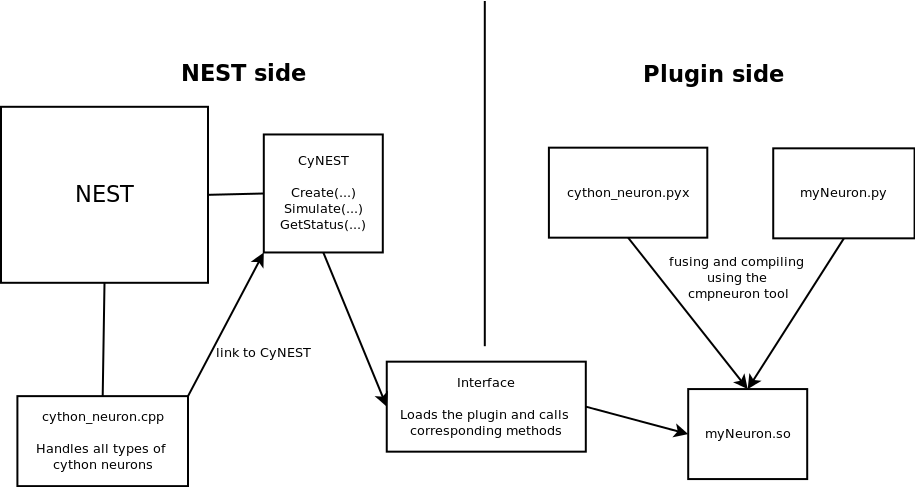
\includegraphics[width=0.92\textwidth]{Ressources/Interface_Structure}
\caption{Interface Structure}
\end{center}
\end{figure}

Figure 1 shows that structure as a diagram. One can see that there's a direct link between cython\_neuron.cpp and CyNEST (normally the two parts cannot directly communicate, but a link is necessary and has been created using static pointers). The interface is placed between CyNEST and the plugin. \\
Let's admit that during a simulation, the update method of a neuron is called (a very likely situation!) and that this neuron is a custom one. The information flow is the following: NEST calls the update method of cython\_neuron.cpp, which through the direct link calls the CyNEST update function. This one uses the interface to call the previously loaded neuron update method inside that plugin file. We can actually say the CyNEST update method is somehow already a part of the interface.\\
During the next sections, the most important regions of the diagram will be covered in much greater detail, so that the reader can have insight into the subtle details and concepts that populate this innovative feature of NEST.

\section{C++ Side}
The fourth section of this document will describe in greater detail the implementation of the general cython neuron handler class, which is responsible for creating new neurons of a certain custom type, handling general events and calling the corresponding plugin functions (calibrate, update, ect...).

\subsection{Neuron Registration}
When creating a new neuron object in the Python terminal by typing\\ \emph{cynest.Create("myneuron")}, NEST will search that particular model among its classes. But how to know if a model has a corresponding class (i.e., if it exists)? The \emph{models/modelsmodule.cpp} class provides the answer. Every new model is registered in the \textbf{models dictionary}, so that when the previous method is called, NEST just checks in this dictionary, looks for a particular model and creates the corresponding class object.\\
In order to register a new model, a code such this has to be written :
\begin{verbatim}
	register_model<iaf_cond_alpha>(net_, "iaf_cond_alpha");
\end{verbatim}
Here, the first \emph{iaf\_cond\_alpha} corresponds to the class name, whereas the second one corresponds to the string pointing to that particular class.\\
All of that implies that when a new custom neuron is added, it must be dynamically registered. This can be achieved by looking for .so files in the cython models folder. Note that when NEST is installed, in the main location there's a folder named \emph{cython\_models} containing the custom created neurons. In fact, after a new neuron has been created, it must be placed there.\\
Therefore, NEST must check for .so files, retrieve their names (of course without the exension) and  register new models giving as class \emph{cython\_neuron} and string the .so file name, like this:
\begin{verbatim}
	register_model<cython_neuron>(net_, file_name);
\end{verbatim}
For more information, look to the \emph{ModelsModule::addCythonNeurons()} method contained in the \emph{models/modelsmodule.cpp} file.

\subsection{General Handler - CyNEST link}
In order to make the overall system work, there is no need for a plugin neuron to implement the totality of the normal neuron methods. The only ones for which a redefinition is mandatory are:
\begin{itemize}
\item Calibrate()
\item Update()
\item GetStatus()
\item SetStatus()
\end{itemize}

Event handling, such as spikes or currents incoming, is enough straightforward to be handled in the \emph{cython\_neuron} class in a general way. Here's an example :
\begin{verbatim}
void nest::cython_neuron::handle(CurrentEvent& e)
{
  assert(e.get_delay() > 0);

  const double_t I = e.get_current();
  const double_t w = e.get_weight();

  // add weighted current; HEP 2002-10-04
  B_.currents_.add_value(e.get_rel_delivery_steps(
                       network()->get_slice_origin()), w * I);
}
\end{verbatim}
However, the previous exposed functions are contained in the plugin neuron and must be called from the C++ class.\\
When dealing with a plugin system, care must be taken to the portability problem. Even if a .so file has been compiled on a machine, maybe it won't work on another one because of the different architectures.\\
Even worse is the Python case: the neuron .so file isn't a normal C or C++ shared library, but a mix of compiled Python and C. Therefore many operations have to be performed when loading such a library, because one has to deal with the Global Lock Interpreter and other annoying Python concepts. Luckily, Cython enables to very easily load files like that without taking into account the low level details.\\
Since NEST already uses Cython for the high level API (CyNEST), the bridge between the general handler and the plugin neuron will be this interface. But how to access functions of CyNEST from this C++ class? The answer is using static function pointers. At the starting of NEST, the high API  will fill these pointers with its own functions, but these pointers are also accessible from the general handler, and since finally the CyNEST is compiled into C++, everything can work. Note that in order everything to work fine, \textbf{at least Cython 0.18 must be installed}. \\ \\
These pointers are situated in the \emph{cynest/buffer.h} file, inside the \emph{CythonEntry} class:
\begin{verbatim}
static void* cInit;
static void* cCalibrate;
static void* cUpdate;
static void* cSetStatus;
static void* cGetStatus;
static void* cStdVars;
static void* cDestroy;
\end{verbatim}
In order to get or set one of these, some methods are available (only one pointer is shown) :
\begin{verbatim}
void putInit(void* value) {
    CythonEntry::cInit = value;
}
void* getInit() {
    return CythonEntry::cInit;
}
\end{verbatim}
Note that it is necessary to make the pointer accessible only through methods. In fact, whereas on the C++ side there's no major problem as it can be accessed directly by the variable name, Cython has some restrictions that must be respected.\\

Before a neuron can call one of these functions, the corresponding pointers must be retrieved, calling methods like \emph{getInit()}, which is performed during neuron initialization. The method \emph{cython\_neuron::initSharedObjects} does this (here's shown the Calibrate functions) :
\begin{verbatim}
void* resultCalibrate = cEntry.getCalibrate();
cythonCalibrate = (void (*)(std::string, int, Datum*))resultCalibrate;
\end{verbatim}
The neuron will then call the \emph{cythonInit} function, which will initialize the neuron on the Cython side, and the \emph{cythonStdVars} function, which will pass the Standard Parameters to the other side. Standard Parameters use and the exact behaviour of these functions will be explained in later sections. \\
The only thing to know is that \emph{cythonInit} will return a neuron pointer, which is usefull to identify an exact neuron among others of the same type. Therefore, for each call to the cython functions, the neuron type and the id are mandatory. Here's an example within the Update method:\\ \\
\begin{verbatim}
for ( long_t lag = from ; lag < to ; ++lag )
  {
    (*state_)[names::in_spikes]=B_.in_spikes_.get_value(lag);
    (*state_)[names::ex_spikes]=B_.ex_spikes_.get_value(lag);
    (*state_)[names::currents]=B_.currents_.get_value(lag);
    (*state_)[names::t_lag]=lag;


    if(cythonUpdate != NULL) {
    	  cythonUpdate(name, neuronID);   // call shared object
    }
    ...

    // surely exists
    spike_emission = (*state_)[names::spike];

    // threshold crossing
    if (spike_emission)
    {
      ...
    }
    ...
  }
\end{verbatim}
As one can see, the \emph{cythonUpdate} function only needs the neuron type and the id. The \emph{state\_} members contains the totality of neuron parameters and is passed to the \emph{cythonInit} function in order to fill the corresponding cython neuron. In fact, for every neuron on the C++ side, there's a corresponding neuron on the Cython side (identified by the neuron type and id). This way, when the C++ neuron will call the Cython one, this latter will already have all the needed parameters, without asking for them.

\subsection{Standard Parameters}
When a neuron calls one of the Cython functions, such as \emph{cythonCalibrate} or \emph{cythonUpdate}, the parameters contained in \emph{status\_} have to be passed to the corresponding cython neuron. The naïve approach of doing that is by copying them into the cython neuron, calling the corresponding function and retry them back.\\
This could work for \emph{cythonCalibare}, but not for \emph{cythonUpdate} as it is called many times and this approach would slow down the system. \\
Furthermore, as one can realize, during a simulation the only important constantly updated parameters by the C++ neuron are :\\
\begin{itemize}
\item currents
\item in\_spikes
\item ex\_spikes
\item t\_lag
\item spike
\end{itemize}
These are called \textbf{Standard Parameters} and are the only one worth copying in the Cython neuron before calling the corresponding function.\\
A good way of speeding up the parameter passing is by giving to the Cython neuron direct pointers to these values, as one can see:
\begin{verbatim}
IntegerDatum* sI = (IntegerDatum*)(*state_)[names::spike].datum();
...
cythonStdVars(get_name(), neuronID, sI->get_p_val(), isD->get_p_val(), 
     esD->get_p_val(), cD->get_p_val(), lI->get_p_val());
\end{verbatim}
Therefore, the Cython neuron will change the values pointed by these pointers without making any copy.\\
However, it is sometimes important to set or retrieve the totality of parameters and this is done during \emph{cythonSetStatus}, \emph{cythonGetStatus} and \emph{cythonCalibrate}.
More information is detailed in the following section.
\section{CyNEST Side}
This section will deal with the Cython side of the project, which has to load the shared file representing the neuron, call all its functions and passing parameters.
\subsection{C++ - Cython Interface}
Cython has a mechanism that allow one to interface C++ classes with Cython code. This is essential because this side has to fill the pointers previously presented.
The file \emph{cynest/classes.pyd} represents this interface and looks like:
\begin{verbatim}
cdef extern from "buffer.h":
    cdef cppclass CythonEntry:
        CythonEntry()
        void putInit(void* value)
        void* getInit()
        void putCalibrate(void* value)
        ...
\end{verbatim}
The following step is to create for each one of these classes, a corresponding wrapping class callable from any Cython code.
\subsection{Filling the pointers}
The wrapper class for \emph{CythonEntry} is situated in the \emph{cynest/dynamicneuronsync.pyx} file and looks like :
\begin{verbatim}
cdef class CythonEntry:
    cdef classes.CythonEntry *thisptr
    def __cinit__(self):
        self.thisptr= new classes.CythonEntry()
        
    def __dealloc__(self):
        del self.thisptr

    cdef void putInit(self, void* value):
        self.thisptr.putInit(value)
    
    cdef void* getInit(self):
        return self.thisptr.getInit()

    cdef void putCalibrate(self, void* value):
        self.thisptr.putCalibrate(value)
    ...
\end{verbatim}
In order to fill the function pointers, one just has to call \emph{putInit}, \emph{putCalibrate} and so on. This is accomplished by the \emph{cynest/kernel.pyx} file by just creating a new \emph{CyrthonEntry} object, calling one of these methods and giving to the pointer another Cython method. Note that this is done during the initialization of CyNEST.
\subsection{Neurons creation}
When a user uses CyNEST within a Python terminal and writes \emph{cynest.Create("myneuron")}, the software must check if the neuron exists and whether it's one of the special cython neurons. This is the purpose of the \emph{processNeuronCreation} function, found in the \emph{cynest/dynamicneuronsync.pyx} file. It's mission is to check if a shared file corresponding to that neuron is present and load it:
\begin{verbatim}
def processNeuronCreation(cmd):
    n = returnNeuronName(cmd)
    if n is not "":
        nList = getDynamicNeuronsName()
        if n in nList and not loadedNeurons.has_key(n):
             libc = PyDLL(spFct.getModelsFolder() + "/" + n + ".so")
             exec("libc.init" + n + "()")
             loadedNeurons[n] = libc
             ...
\end{verbatim}
Note that in the last version this method has been splitted into two parts for accounting loadings during other parts of the code. However, it has been kept together in order to give a global view.\\
A very important point to realize is that, differently from Python, since Cython is a compiled code it cannot dynamically load another file, for instance using \emph{import myneuron}. This is a huge drawback that will limit performances and coding style. The only way of dynamically loading a file is by using the \emph{ctypes} library included in Python.\\
This is what has been done in the previous code by calling\emph{... = PyDLL(...)}. The picture depicting the structure of the project shows that on the plugin side, a file named \emph{cython\_neuron.pyx} is mixed with the user written neuron. This is true and the final output becomes a shared file. This latter will contain interface functions callable from other code (in this case the Cython side of the project).\\ \\
However, since ctypes has been created for Python, it cannot be used in a proper way with Cython, mostly when dealing with pointers. As an example, Cython code cannot direct pass a pointer to a shared file function, but must make a copy of the pointed value in a special ctypes object, create a corresponding ctypes pointer, make all the necessary computations and retrieve that value from the ctypes pointer.\\ 
This makes the Standard Parameters approach very limitative, loosing a lot of its original benefits.
\subsection{Neuron basic functions}
This section will explain the behaviour of the neuron functions callable from the C++ side of the project. These are:
\begin{itemize}
\item cInit: this function, called by \emph{cythonInit}, will initialize the neuron. The steps are:  call the \emph{createNeuorn()} method of the plugin file, append a new entry in a special table created to store the Standard Parameters and synchronize the neuron. This is done by calling the \emph{setNeuronMembers} and \emph{retrieveNeuronMembers} functions, therefore enabling the two neurons (one on the C++ side and the other on the Cython side) to have exactly the same number of parameters. Finally, the function returns the neuron id.

\item cCalibrate: this function will give to the Cython neuron the C++ neuron parameters, then call the corresponding function (\emph{calibrate}) and retrieve the updated parameters.


\item cSetStatus: this function will give to the Cython neuron the C++ neuron parameters, then call the corresponding function (\emph{setStatus}) and retrieve the updated parameters. In fact, a neuron could adjust some of them relatively to other ones.


\item cGetStatus: this will call the corresponding function (\emph{getStatus}) and retrieve the updated parameters. During an execution, the only time the non Standard Parameters are used is when the user calls the \emph{cynest.GetStatus(...)} command on the Python terminal. That's why it is important to retrieve them.


\item cStdVars: this function will save the Standard Parameters pointers in a special double array object of type \emph{StandardParams}.

\item cUpdate: this is the most important function. Here's the implementation:
\begin{verbatim}
cdef void cUpdate(string nName, int neuronID) with gil:
    ...
    cdef StandardParams sp = stdParams[neuronName][neuronID]
    loadedNeurons[neuronName].setStdVars(neuronID, sp.spike[0], 
    	    sp.in_spikes[0], sp.ex_spikes[0], sp.currents[0], sp.lag[0])

    loadedNeurons[neuronName].update(neuronID)

    loadedNeurons[neuronName].getStdVars(neuronID, sIR, isDR, 
         esDR, cDR, lIR)
    sp.spike[0] = sI.value
    sp.in_spikes[0] = isD.value
    ...
\end{verbatim}
The logic of the function is very simple : first the Standard Parameters are passed to the shared file, by value and not by pointer, then the \emph{update} function is called. However, the dealing with the retrieving, the special ctypes objects are used. Finally, when every computation has been performed, the ctypes objects values are copied in the pointed values. As previously said, this is a huge limitation of the mechanism.
\end{itemize}

\subsection{Parameters passing}
As explained in the last subsection, two possible modes of parameter passing are possible: Standard Parameters and nn Standard Parameters. Let's see how they work:
\begin{itemize}
\item Standard Parameters:\\
This is done by calling the \emph{setStdVars} and \emph{getStdVars} in the \emph{cUpdate} function, as previosuly said. But where are these functions? These are situated in the \emph{cmpneuron/cython \_neuron.pyx} file and are very straightforward (the way this file is compiled is discussed in the following section):
\begin{verbatim}
cdef public void setStdVars(int neuronID, long spike, double in_spikes, 
            double ex_spikes, double currents, long lag) with gil:
    neurons[neuronID].spike = spike
    neurons[neuronID].in_spikes = in_spikes
    neurons[neuronID].ex_spikes = ex_spikes
    neurons[neuronID].currents = currents
    neurons[neuronID].t_lag = lag


cdef public void getStdVars(int neuronID, long* spike, double* in_spikes, 
            double* ex_spikes, double* currents, long* lag) with gil:
    spike[0] = neurons[neuronID].spike
    in_spikes[0] = neurons[neuronID].in_spikes
    ex_spikes[0] = neurons[neuronID].ex_spikes
    currents[0] = neurons[neuronID].currents
    lag[0] = neurons[neuronID].t_lag
\end{verbatim}
The first one just copies the arguments to a special array. This array represents the counterpart neurons of the C++ ones.\\
The second function just copies to Standard parameters contained in the neuron to the pointed values.
\item Non Standard Parameters:\\
This exchange mechanism is a little more tricky. It's implemented through the functions \emph{setNeuronMembers} and \emph{retrieveNeuronMembers}. Here's the code for the first one:
\begin{verbatim}
cdef void setNeuronMembers(bytes neuronName, int neuronID, 
        classes.Datum* parameters) with gil:
    cdef dict members = <dict>converter.datumToObject(parameters)
    loadedNeurons[neuronName].setNeuronParams.argtypes = [c_int, py_object]
    loadedNeurons[neuronName].setNeuronParams(neuronID, py_object(members))
\end{verbatim}
The first line of the function is a conversion. As one can see, the function arguments contain a special \emph{Datum} object. This comes from the C++ side and represents an SLI object (can contain integers, doubles, booleans, lists, dictionaries and every other builtin type). In this case it is a \emph{DictionaryDatum} representing the totality of neuron parameters.\\
The \emph{converter} is a wrapper object of type \emph{DataConverter} and its role is to transform a \emph{Datum} into a Python object, in this case a dictionary. The converters this object wrap are CyNEST parts, therefore for more information see the CyNEST doc.\\
Once the dictionary is ready, this is passed to the \emph{setneuronParams} function contained in tghe \emph{cmpneuron/cython\_neuron.pyx} file, which will simply loop over the dictionary and add the corresponding values to theneuron fields.\\ \\


The retrieving of the neuron parameters works quite similarly:
\begin{verbatim}
cdef void retrieveNeuronMembers(bytes neuronName, int neuronID, 
        classes.Datum* parameters) with gil:
    ...
    cdef classes.Datum* members = converter.objectToDatum
           (loadedNeurons[neuronName].getNeuronParams(neuronID))
    converter.updateDictionary(members, parameters)
    ...
\end{verbatim}
The converter transforms the retrieved object (which is just a dictionary containing all the neuron parameters on the plugin side, except for those beginning with '\_'. Seet next section for more explanations) into a \emph{Datum} pointer. This latter will then update the real \emph{Datum} object used on the C++ side.
\end{itemize}
\subsection{Special Functions}
Sometimes, a neuron model needs some special information from the system, such as simulation parameters. The values represent time units, simulation delays, ect...\\
Therefore, the system has to enable the final user to access these variables and this is achieved by what is called \textbf{Special Functions}. The class \emph{SpecialFunctions} contained in the file \emph{cynest/buffer.h} possesses all the necessary to provide that functionality :
\begin{verbatim}
class SpecialFunctions {
private:
    Time createTime(int inputType, long longInputValue, double doubleInputValue) {
        ...
    }

public:
    double get_ms(int inputType, long longInputValue, double doubleInputValue) {
        ...
    }

    long get_tics_or_steps(int inputType, int outputType, 
          long longInputValue, double doubleInputValue) {
        ...
    }

    unsigned int get_scheduler_value(int outputValue, unsigned int arg) {
        ...
    }

};
\end{verbatim}
The purpose of this system is to emulate a command such as :
\begin{verbatim}
    Scheduler::get_min_delay()
or
    Time::get_resolution().get_ms()
or
    Time::step(steps).get_tics()
\end{verbatim}
The first line is emulated through the function \emph{get\_scheduler\_value} choosing between some possibilities by setting the \emph{outputValue} argument to:
\begin{itemize}
\item 0 for \emph{Scheduler::get\_modulo(arg)}
\item 1 for \emph{Scheduler::get\_slice\_modulo(arg)}
\item 2 for \emph{Scheduler::get\_min\_delay()}
\item 3 for \emph{Scheduler::get\_max\_delay()}
\end{itemize}
The second and third lines are emulated using a slight different mechanism. The user can specify the unit of the Time class creation (which corresponds to the unit in which the neural network is simulated), via the \emph{SpecialFunctions::createTime} method, following these rules:
\begin{itemize}
\item 0 for Time::get\_resolution()
\item 1 for Time(Time::tic(tics))
\item 2 for Time(Time::step(steps))
\item 3 for Time(Time::ms(ms))
\item 4 for Time(Time::ms\_stamp(ms\_stamp))
\end{itemize}
Note that since tics, steps are integer values and ms, ms\_stamp are double values, the method needs two different arguments, choosen with respect to \emph{inputType}.\\
Once the Time object has been created, the \emph{SpecialFunctions::get\_ms} and \emph{SpecialFunctions::get\_tics\_or\_steps} methods will return the choosen unit.
For the latter method, the output unit has to be choosen, giving 1 for tics and 2 for steps.\\ \\
The next step is to interface with Cython and this is done in the \emph{cynest/classes.pyx} file:
\begin{verbatim}
cdef cppclass SpecialFunctions:
    SpecialFunctions()
    double get_ms(int, long, double)
    long get_tics_or_steps(int, int, long, double)
    unsigned int get_scheduler_value(int, unsigned int)
\end{verbatim}
This class will be of course wrapped in another one. The final purpose is to a pointer corresponding to each one of these methods to the plugin neuron, and this is achieved using ctypes, with the following code:
\begin{verbatim}
def get_ms(arg1, arg2, arg3):
    return spFct.get_ms(arg1, arg2, arg3)
...
GETMSFUNC = CFUNCTYPE(c_double, c_int, c_long, c_double)
...
getmsFCT = GETMSFUNC(get_ms)
...
def processNeuronCreation(cmd):
   ...
   loadedNeurons[n].putSpecialFunctions(getmsFCT, ...)
\end{verbatim}
Where \emph{spFct} is a \emph{SpecialFunction} object (the wrapper class) and \emph{putSpecialFunctions} is a method contained in the \emph{cmpneuron/cython\_neuron.pyx} file.
\\
The user will finally access these functionalities by calling the following commands:
\begin{verbatim}
def get_ms_on_resolution(self):
    return spFct.get_msFct(0, -1, -1)

def get_ms_on_tics(self, tics):
    return spFct.get_msFct(1, tics, -1)

def get_ms_on_steps(self, steps):
    return spFct.get_msFct(2, steps, -1)
...
\end{verbatim}
There are many more (15 in total). See the user documentation or the code for the complete list.
Note that these functions are callable from the base \emph{Neuron} class (see next section) and their behaviour is quite simple : they just call the pointer functions previously setted giving the correct arguments. Also note that \emph{spFct} is a different object from the other one since we are in a different file. That object just holds the function pointers setted by \emph{putSpecialFunctions}.
\section{Compiling the Plugin Neuron}
Once the CyNEST can correctly recognize new cython neurons, the final step is to create shared files. This is the work of the \textbf{cmpneuron} tool. It takes a .py file and returns after compilation a .so file, corresponding to the loadable neuron. See the cmpneuron documentation for more detail about the utilization.\\ \\
This section will briefly explain the steps this tool performs in order to compile the neuron.\\
The idea is simple: the template file (\emph{cython\_neuron.pyx}) contains the base, other than all the previously exposed functions, the base class Neuron. cmpneuron will copy the user class, extending from Neuron, in the file and create objects of this type.\\ \\ 
Let's admit a user has written a new neuron, called MyNeuron in the MyNeuron.py file. Then cmpneuron will perform the following steps:
\begin{itemize}
\item Copying of the files \emph{cython\_neuron.pyx} and \emph{setup.py} (contained in the executable directory) to the user directory (the one containing the user .py file).
\item Modification of the \emph{setup.py} file, by replacing the line
\begin{verbatim}
    ext_modules = [Extension("cython_neuron", ["cython_neuron.pyx"])]
\end{verbatim}
with
\begin{verbatim}
    ext_modules = [Extension("MyNeuron", ["cython_neuron.pyx"])]
\end{verbatim}
\item Modification of the template \emph{cython\_neuron.pyx} file by adding the content of \emph{MyNeuron.py} to a special location, delimited by some anchoring symbols (see the template). At the location where the actual neuron is created, the tool will also modify the line (with anchoring symbols) like this:
\begin{verbatim}
    n = MyNeuron()
\end{verbatim}
\item Compilation of the modified files by invoking Cython with this command:
\begin{verbatim}
    python setup.py build_ext --inplace
\end{verbatim}
\item Deletion of intermediate files.
\end{itemize}
Once the shared file is created, it can be put by the user in the special folder \emph{NEST\_Folder/cython\_models}, where NEST\_Folder is the folder in which CyNEST has been installed.
\section{Performances}
The system has been tested during a single-threaded simulation of 40 ms concerning over 1000 randomly connected neurons and compared to their native and SLI counterparts. The results are:
\begin{itemize}
\item Native neuron: realtime factor is 0.3254
\item SLI neuron: realtime factor is 0.0046
\item Cython neuron: realtime factor is 0.0049
\end{itemize}
We can therefore conclude that the Cython neuron is 66.38 slower than the native version, whereas it is approximatively the same as the SLI neuron.\\
Note that during different test trials, values could slightly change because of the random factor introduced in the network.\\
Why is the system so slow? Several reasons can explain that:
\begin{itemize}
\item Parameter passing is extremely slow and seems to be the major bottleneck. As previously explained, there is any possibility to directly pass a C pointer to a dynamically loaded file, but one should use ctypes pointers instead, which are slow (since Python is used).
\item The neuron itself is another important bottleneck! Since the user can write the neuron in Python, Cython cannot optimize too much and has to import the entire Python machinery.
\end{itemize}
\section{Tests}
The project has undergone an great amount of tests and passed everyone of them. These are located in the \emph{testsuite/cythontests} folder. \\
Basically, three tests have been created :
\begin{itemize}
\item test\_create : these bunch of tests check if a model is correctly created, if dictionary parameters are correctly set and if models are connected the good way.
\item test\_status : they check the \emph{GetDefaults}, \emph{SetDefaults}, \emph{GetStatus} and \emph{SetStatus} methods.
\item test\_use : the aim is to check the parameters type consistency. All possible parameter types are created, a simulation started, and then retrieved. Custom objects and functions are not available as types and this is also checked.
\end{itemize}
\section{Problems and Difficulties}
The overall project wasn't so difficult because Cython hides a lot of low level details important when dealing with shared libraries. The main problem was to understand how Cython works and correctly use its syntax, which is not as simple as it seems.\\
But before even beginning the project, a great amount of work as been accomplished in order to understand how NEST works and how all its classes are related.\\
Some little encountered problems were:
\begin{itemize}
\item Installing the good version. Package managers don't actually know which is the latest Cython release, so one must care of installing the one on the website.
\item The Global Lock Interpreter has to be used in order to maintain cython data persistent. This is done using the code \emph{with gil} after a function declaration.
\item C++ pointers cannot be directly given to shared object functions and another solution has to be found.
\item The Cython syntax can be confusing, making sometimes mandatory to write code in a less elegant way. As an example, the \emph{Cannot convert Python object to...} error is a very common and annoying one.
\item Some global objects are not persistent (do not store the last updated value) during the program execution and have to be placed inside classes in order to be.
\end{itemize}
\section{Conclusion}
At the end of the project, the system works quite well and implements the suited features.\\
However, as previously stated, it has some major limitations, the main one being the slowness. In a previous version, one could create custom objects inside the neuron, but the field names have to start with "\_", otherwise an error occurs. This problem has been recently fixed and that's now possible to choose if a neuron field is public or private by beginning its name with \_ or not. If a custom type field doesn't have a private name, it is simply ignored when passed to NEST.\\
Another main limitation is represented by the proposed neuron accesses: there is no way to handle events and access some (maybe) usefull system fields. This should be implemented in the future. \\ \\ \\
An important question therefore arises: is there a better way to propose more or less the same 
functionalities, but making the neuron much faster?\\
Maybe yes! It could be possible, but the price would be the syntax reduction. The neuron should become a "highly configurable" one. The user should configure it by using a very simple language which enables:
\begin{itemize}
\item Fields creation, but only of builtin types (integers, booleans, doubles and strings).
\item Basic operations (+, -, *, /, \%) for formulas evaluation.
\item Basic control flow structures (if\ldots else, while\ldots).
\item External mathematical functions, provided by the language.
\item Special external functions or fields, provided by the language, which will call NEST functions or access NEST parameters.
\end{itemize}
That should be compiled in a "Java-bytecode"-like language, which would be loaded by the neuron before the simulation and executed using a buffer for instructions and a stack for variables.\\
Such a solution should be much faster than their Cython counterpart.
\end{document}